\documentclass[letterpaper,10pt,twoside]{amsart}
%\usepackage{extsizes}
%%\usepackage{standalone} % For getting .tex files into separated files and look at the compilation.
%\usepackage[utf8]{inputenc}
%\usepackage{enumitem}
%\setlist{nosep}
%\usepackage{graphicx}
\usepackage{amsmath,amssymb,amsfonts,amsthm}
%\usepackage{biblatex}
\usepackage{tikz-cd}
\usepackage[margin=0.9in,
left=1in,%
right=1in,%
top=1.25in,%
bottom=1.25in
]{geometry}	
\usepackage{stmaryrd} %For mapsfrom.

\usepackage[colorinlistoftodos]{todonotes} %For todonotes.
\usepackage{tcolorbox}
\usepackage{longtable}
\usepackage{booktabs}

%\usepackage{totcount}
%\regtotcounter{theorem}


%\usepackage{minitoc} %To get a table of contents for each chapter.

\usepackage{lscape}

\usepackage{xstring}


%\usepackage[affil-it]{authblk}
%\usepackage{setspace} %For good space between ToC entries.

%\addtolength{\topmargin}{-.875in}

%%%%------ Fonts-------------
%\usepackage{fontspec}
%\setmainfont{QTHandwriting}
% \usepackage{boisik}
% \usepackage[OT1]{fontenc}

% \usepackage{mlmodern}
% \usepackage[T1]{fontenc}
% \usepackage{palatino}
%--------------------------------


\usepackage{quiver}
\usepackage{bm}
\usepackage{fancyhdr}
\usepackage{mathrsfs}
\usepackage{amsbsy}
%\usepackage{titlesec}
\usepackage{yhmath}
\usepackage{pifont}

%Hyperref Settings------
\usepackage{hyperref}
\usepackage{xcolor}
\hypersetup{
	colorlinks=true,
	linkcolor={blue},
	citecolor={blue},
	anchorcolor={blue}
}

%Macro for acts in proofs
\newenvironment{act}[2]{\begin{center}
		\textbf{Act #1} : \textit{#2}
	\end{center}
}

%Font packages:-


\usepackage[scr=euler,scrscaled=1.05]{mathalfa} %For different symbol for Categories
\usepackage{dashbox}
\usepackage{euscript}

%TITLE:-
\title{Smooth and \'Etale Morphisms}
\date{\today}

%\author{Animesh Renanse}

%MACROS:-

%1. Spectrum of a ring
\newcommand{\spec}[1]{{\fontfamily{lmss}\selectfont 
		\text{\rm Spec}\left(#1\right )
}}


%2. Categories
%\newcommand{\cat}[1]{{\fontfamily{lmss}\selectfont 
		%		\text{\rm\textbf{#1}}
		%}}
\newcommand{\cat}[1]{\mathscr{\StrChar{#1}{1}}\StrGobbleLeft{#1}{1}}
%\newcommand{\opcat}[1]{{\fontfamily{lmss}\selectfont 
		%		\text{\rm\textbf{#1}}^{\text{\rm op}}
		%}}
\newcommand{\opcat}[1]{\cat{#1}^{\text{op}}}
%3. Homsets
\newcommand{\homset}[3]{{\fontfamily{lmss}\selectfont 
		\text{\rm Hom}_{#1}\left (#2,#3\right )
}}
%4. Chain complexes
\newcommand{\Ch}[1]{\cat{Ch}\left (#1\right )}
%5. Kernel and Image and CoKernel and CoImage
\newcommand{\Ker}[1]{{\fontfamily{lmss}\selectfont 
		\text{\rm Ker}\left (#1\right )
}}
\newcommand{\Image}[1]{{\fontfamily{lmss}\selectfont 
		\text{\rm Im}\left (#1\right )
}}
\newcommand{\CoKer}[1]{{\fontfamily{lmss}\selectfont 
		\text{\rm CoKer}\left (#1\right )
}}
\newcommand{\CoIm}[1]{{\fontfamily{lmss}\selectfont 
		\text{\rm CoIm}\left (#1\right )
}}
%6. Isomorphism
\newcommand{\isom}{\cong}
%7. Bold blank
\newcommand{\blank}{\bm{-}}
%8. Restriction
\newcommand{\rest}[2]{\left. { #1 }\right \vert_{#2}}
%9. Submodule
\newcommand{\Sub}[1]{\text{\rm Sub}\left (#1\right )}
%10. Sp
\newcommand{\Sp}[1]{\text{\rm Sp}\left (#1\right )}
%11. Open Sets
\newcommand{\Op}[1]{\mathcal{O}_{#1}}
%12. Reals
\newcommand{\R}[0]{\mathbb{R}}
%13. Inner Product
\newcommand{\ip}[2]{\langle #1,#2 \rangle}
%14. Norm
\newcommand{\norm}[1]{\Vert #1 \Vert}
%15. Absolute
\newcommand{\abs}[1]{\left\vert #1 \right \vert}
%16. Ideals
\newcommand{\ideal}[1]{\mathfrak{#1}}
%17. Generated
\newcommand{\gen}[1]{\langle #1 \rangle}
%18. Integers
\newcommand{\Z}{\mathbb{Z}}
%19. Identity
\newcommand{\id}{{\fontfamily{lmss}\selectfont 
		\text{\rm id}
}}
%20. Tensor
\newcommand{\tens}{\otimes}
\newcommand{\btens}{\bigotimes}
%21. Annihilator
\newcommand{\Ann}[0]{{{\fontfamily{lmss}\selectfont 
			\text{\rm Ann}
}}}
%22. Naturals, Rationals.
\newcommand{\N}{\mathbb{N}}
\newcommand{\Q}{\mathbb{Q}}
%23. Image
\newcommand{\image}{{\fontfamily{lmss}\selectfont 
		\text{\rm Image}
}}
%24. Direct sum
\newcommand{\bdsum}{\bigoplus}
%25. Union and Intersection
\newcommand{\union}{\cup}
\newcommand{\intrs}{\cap}
\newcommand{\bunion}{\bigcup}
\newcommand{\bintrs}{\bigcap}
%26. Inverse
\newcommand{\inv}[1]{\left (#1\right )^{-1}}
%27. Radical
\newcommand{\rad}[1]{\sqrt{#1}}
%28. Maximal spectrum
\newcommand{\mspec}[1]{{\fontfamily{lmss}\selectfont 
		\text{\rm mSpec}\left (#1\right )
}}
%29. Support
\newcommand{\supp}[1]{{\fontfamily{lmss}\selectfont 
		\text{\rm Supp} \left (#1\right )
}}
%30. Structure sheaf
\newcommand{\ssh}{\mathscr{O}}
%31. General sheaf
\newcommand{\sh}[1]{\mathscr{#1}}
%32. Limit and colimit and usual limit
\renewcommand{\lim}{\varprojlim}
\newcommand{\colim}{\varinjlim}
\newcommand{\ulim}{\text{\rm lim}}
%33. Point
\newcommand{\pt}{\text{\rm pt.}}
%34. Complex numbers
\newcommand{\C}{\mathbb{C}}
%35. Associated prime ideals.
\newcommand{\Ass}[1]{{\fontfamily{lmss}\selectfont 
		\text{\rm Ass} \left (#1\right )
}}
%36. Holomorphic 
\newcommand{\hol}{\text{\rm hol}}
%37. Widetilde
\newcommand{\wt}[1]{\widetilde{#1}}
%38. Index of a curve
\newcommand{\ind}[1]{{\fontfamily{lmss}\selectfont 
		\text{\rm ind} \left (#1\right )
}}
%39. Automorphism group
\newcommand{\Aut}[1]{{\fontfamily{lmss}\selectfont 
		\text{\rm Aut} \left (#1\right )
}}
%40. Affine space
\newcommand{\A}{\mathbb{A}}
%41. Finite
\newcommand{\fin}{\text{\rm fin}}
%42. Short hyphen
\DeclareMathSymbol{\hyp}{\mathord}{AMSa}{"39}
%43. Interior
\newcommand{\Int}{{\fontfamily{lmss}\selectfont 
		\text{\rm Int}
}}
%44. Trace
\newcommand{\Tr}{{\fontfamily{lmss}\selectfont 
		\text{\rm Tr}
}}
%45. Diagonal
\newcommand{\diag}{{\fontfamily{lmss}\selectfont 
		\text{\rm diag}
}}
%46. Projective space
\DeclareMathOperator{\pr}{\mathbb{P}}
%47. Proj
\newcommand{\proj}[0]{{\fontfamily{lmss}\selectfont 
		\text{\rm Proj}
}}
%48. Simplex category
\newcommand{\dcat}[0]{\boldsymbol{\Delta}}
%49. Presheaf cateogry
\newcommand{\psh}[1]{\widehat{\cat{#1}}}
%50. Yoneda embedding
\newcommand{\yon}[0]{{\fontfamily{lmss}\selectfont 
		\text{\rm Yon}
}}
%51. image
\renewcommand{\image}[1]{{\fontfamily{lmss}\selectfont 
		\text{\rm im}\left(#1\right)
}}
%52. Index of a complex curve
\newcommand{\Ind}[0]{{\fontfamily{lmss}\selectfont 
		\text{\rm Ind}
}}
%53. Residues
\newcommand{\res}[0]{{\fontfamily{lmss}\selectfont 
		\text{\rm res}
}}
%54. Blackboard P
\renewcommand{\P}[0]{\mathbb{P}}
%55. Chain and cochain complexes
\newcommand{\ch}[1]{\mathrm{Ch}\left(\cat{#1}\right)}
\newcommand{\cch}[1]{\mathrm{coCh}\left(\cat{#1}\right)}
%56. Hom sheaf
\newcommand{\shom}[0]{\sh{H}om}
%57. Picard group
\newcommand{\Pic}[0]{{\fontfamily{lmss}\selectfont 
		\text{\rm Pic}
}}
%58. Mathcal
\newcommand{\mc}[1]{\mathcal{#1}}
%59. Set of valuations
\newcommand{\val}[0]{{\fontfamily{lmss}\selectfont 
		\text{\rm Val}
}}
%60. Height of a prime ideal
\newcommand{\height}[0]{{\fontfamily{lmss}\selectfont 
		\text{\rm ht\;}
}}
%60. Coheight of a prime ideal
\newcommand{\coht}[0]{{\fontfamily{lmss}\selectfont 
		\text{\rm coht\;}
}}
%61. Transcendence degree
\newcommand{\trdeg}[0]{{\fontfamily{lmss}\selectfont 
		\text{\rm trdeg\;}
}}
%62. Codimension
\newcommand{\codim}[0]{{\fontfamily{lmss}\selectfont 
		\text{\rm codim\;}
}}
%63. Divisors
\newcommand{\Div}{{\fontfamily{lmss}\selectfont 
		\text{\rm Div\;}
}}
%64. Reduced
\newcommand{\red}{\text{\rm red}}
%65. Internal hom
\newcommand{\ihom}[2]{{\fontfamily{lmss}\selectfont 
		\text{\rm \underline{Hom}}\left (#1,#2\right )
}}
%66. Simplex category
\newcommand{\smplx}{\bm{\Delta}}
%67. Null sets
\newcommand{\Null}{\text{\rm Null}}
%68. Easy \mu
\newcommand{\m}{\mu}
%69. Prime divisors
\newcommand{\Pdiv}{\text{\rm PDiv}}
%70. DVRs
\newcommand{\Dval}{\text{\rm DVal}}
%71. Finite field
\newcommand{\F}{\mathbb{F}}
%72. Sign
\newcommand{\sgn}{\text{\rm sgn}}
%73. Adjoint of a matrix
\newcommand{\Adj}{\text{\rm Adj}}
%74. Simple class
\newcommand{\Simp}{\text{ \rm Simp}}
%75. Blackboard
\newcommand{\bb}[1]{\mathbb{#1}}
%76. Mathscr
\newcommand{\mscr}[1]{\mathscr{#1}}
%77. Divides
\renewcommand{\div}{\vert}
%78. Global spec
\newcommand{\gspec}{\text{\rm \textbf{Spec}}}
%79. Global proj
\newcommand{\gproj}{\text{\rm Proj}}
%80. Map
\newcommand{\Map}{\text{\rm Map}}
%81. Sing
\newcommand{\Sing}{\text{\rm Sing}}
%82. Reals or Complex
\newcommand{\K}{\mathbb{K}}
%83. Ceiling
\newcommand{\ceil}[1]{\left \lceil #1 \right \rceil}
%84. alg
\newcommand{\alg}{\text{\rm alg}}
%85. Frobenius
\newcommand{\Fr}{\text{\rm Fr}}
%86. Characteristic
\newcommand{\charac}{\text{\rm char}}
%87. Galois group
\newcommand{\Gal}[1]{\text{\rm Gal}\left (#1\right )}
%88. Evaluation
\newcommand{\ev}{\text{\rm ev}}
%89. deRham
\newcommand{\dR}{\text{\rm dR}}
%90. Rank
\newcommand{\rk}{\text{\rm rank}}
%91. Acts
\DeclareMathOperator{\acts}{\rotatebox[origin=c]{-90}{$\circlearrowright$}}
%92. Cl
\DeclareMathOperator{\Cl}{\text{\rm Cl}}
%93. Proof ding!
\DeclareMathOperator{\myproof}{\dagger}
%94. Whitehead
\DeclareMathOperator{\Wh}{\text{\rm Wh}}
%95. GL
\DeclareMathOperator{\GL}{\text{\rm GL}}
%96. SL
\DeclareMathOperator{\SL}{\text{\rm SL}}
%97. End
\DeclareMathOperator{\End}{\text{\rm End}}
%98. Steinberg
\DeclareMathOperator{\St}{\text{\rm St}}
%99. Matsumoto
\DeclareMathOperator{\Mat}{\text{\rm Mats}}
%100. Symbols
\DeclareMathOperator{\Symb}{\text{\rm Symb}}
%101. BGL
\DeclareMathOperator{\BGL}{\text{\rm BGL}}
%102. Brauer
\DeclareMathOperator{\Br}{\text{\rm Br}}
%103. Etale
\DeclareMathOperator{\et}{\text{\rm \'et}}
%104. Separable
\DeclareMathOperator{\sep}{\text{\rm sep}}
%105. Blackboard G
\DeclareMathOperator{\G}{\mathbb{G}}
%106. Ext
\DeclareMathOperator{\Ext}{\text{\rm Ext}}
%107. Partial
\DeclareMathOperator{\del}{\partial}
%108. Simplicial Sets
\DeclareMathOperator{\sSet}{s\cat{Set}}
%109. Topological spaces
\DeclareMathOperator{\Top}{\cat{Top}}
%110. Ordinal category
\newcommand{\bD}{\bm{\Delta}}
%111. Opposite
\DeclareMathOperator{\op}{\text{\rm op}}
%112. Category of sets
\DeclareMathOperator{\Set}{\cat{Set}}
%113. Inc
\DeclareMathOperator{\Inc}{\text{\rm Inc}}
%114. Simplicial sphere
\renewcommand{\SS}{\mathbb{S}}
%115. Skeleton
\DeclareMathOperator{\sk}{\text{\rm sk}}
%116. Base ring
\newcommand{\bK}{\bm{K}}
%117. Category of graded coalgebras 
\DeclareMathOperator{\coAlg}{\text{\rm co}\cat{Alg}}
%118. Category of graded coalgebras 
\DeclareMathOperator{\gcoAlg}{\text{\rm gco}\cat{Alg}}
%119. Category of dg coalgebras 
\DeclareMathOperator{\dgcoAlg}{\text{\rm dgco}\cat{Alg}}
%120. Category of dg algebras 
\DeclareMathOperator{\dgAlg}{\text{\rm dg}\cat{Alg}}
%121. Bold Omega
\newcommand{\cobar}{\bm{\Omega}}
%122. \mathfrak{C}
\DeclareMathOperator{\frC}{\mathfrak{C}}
%123. \mathfrak{N}
\DeclareMathOperator{\frN}{\mathfrak{N}}
%124. hTop
\DeclareMathOperator{\hTop}{h\Top}
%125. Cat
\DeclareMathOperator{\Cat}{\cat{Cat}}
%126. sCat
\DeclareMathOperator{\sCat}{s\cat{Cat}}
%127. Presheaf category
\newcommand{\ps}[1]{\widehat{\cat{#1}}}
%128. Necklaces
\DeclareMathOperator{\Neck}{\cat{Neck}}
%129. Simplicial monoids
\DeclareMathOperator{\sMon}{s\cat{Mon}}
%130. Cubical sets
\DeclareMathOperator{\cSet}{c\cat{Set}}
%131. Collapse
\DeclareMathOperator{\collapse}{\searrow}
%132. Formal deformation
\DeclareMathOperator{\fd}{\curvearrowright}
%133. Expansion
\DeclareMathOperator{\expand}{\nearrow}
%134. Base field
\DeclareMathOperator{\basef}{\mathbf{k}}
%135. Chow groups
\DeclareMathOperator{\CH}{\text{\rm CH}}
%136. Etale
\DeclareMathOperator{\etale}{\text{\rm \'et}}
%137. Bun
\DeclareMathOperator{\Bun}{\cat{Bun}}
%138. Isomorphism classes of Torsors
\DeclareMathOperator{\Tors}{\text{\rm Tors}}
%139. Isomorphism classes of vector bundles
\DeclareMathOperator{\Vect}{\text{\rm Vect}}
%141. Grassmannian 
\DeclareMathOperator{\Gr}{\text{\rm Gr}}
%142. PSL
\DeclareMathOperator{\PSL}{\text{\rm PSL}}
%143. Derivations
\DeclareMathOperator{\Der}{\text{\rm Der}}


%Header and Footer style:-
%\pagestyle{fancy}
%\fancyhf{}
%\fancyhead[CO]{{\fontfamily{lmss}\selectfont \ssmall \rightmark}}
%\fancyhead[CE]{{\fontfamily{lmss}\selectfont \ssmall \leftmark}}%Add name instead of date.
%\fancyhead[LE,RO]{{\fontfamily{lmss}\selectfont \ssmall \thepage}}
%\fancyhead[LO,RE]{}
%\fancyfoot[CE,CO]{}
%\fancyfoot[LE,RO]{}
\setlength{\headheight}{15pt}
\renewcommand{\headrulewidth}{0pt}

\usepackage{moresize}



%MATH BACKGROUND DECLARATORS-------------------------------------------------------
\theoremstyle{proposition}
\newtheorem{proposition}{Proposition}[section]

\theoremstyle{definition}
\newtheorem{definition}[proposition]{Definition}

\theoremstyle{theorem}
\newtheorem{theorem}[proposition]{Theorem}

\theoremstyle{definition}
\newtheorem{remark}[proposition]{\textbf{Remark}}

\theoremstyle{definition}
\newtheorem{notation}[proposition]{\textbf{Notation}}

\theoremstyle{definition}
\newtheorem{discussion}[proposition]{\textbf{Discussion}}

\theoremstyle{lemma}
\newtheorem{lemma}[proposition]{\textbf{Lemma}}

\theoremstyle{definition}
\newtheorem{example}[proposition]{\textbf{Example}}

%\theoremstyle{remark}
%\newtheorem*{comment}{\textbf{Comments on Proof Technique}}

\theoremstyle{definition}
\newtheorem{construct}[proposition]{Construction}

\theoremstyle{corollary}
\newtheorem{corollary}[proposition]{Corollary}

\theoremstyle{definition}
\newtheorem{caution}[proposition]{\textbf{Caution}}

%---------------------------------------------------------------------------------
%\setcounter{tocdepth}{2}


%\author[1]{Jesse Kass}


\begin{document}
	\maketitle
	\begin{abstract}
		A smooth manifold is locally diffeomorphic to an open subset of $\R^{n}$. Our goal in this note is to prove the same in the case of rings. One observes immediately that this is far from true in Zariski topology, thus necessitating search of finer topologies on rings. After motivating unramified, \'etale morphisms and coverings, we will introduce smooth homomorphisms of rings as finitely presented flat morphisms for which K\"ahler differentials is locally trivial. At the end, we will see that every smooth homomorphism of rings is \'etale locally given by projection from an affine space, as expected.
%		\begin{enumerate}
%			\item {Motivate by trying to define covering spaces in algebraic geometry. DONE}
%			\item {Define the module of K\"ahler differentials $\Omega_{B/A}$ of a ring homomorphism $A\to B$ [Aso19, Definition 6.2.3.1, Propositions 6.3.1.3, 6.3.4.1]. DONE, except the proof of 6.3.4.1.}
%			\item {Define smooth and \'etale ring homomorphisms [Aso19, §6.2.1, 6.2.2, 6.7.2], and state the equivalent characterization via formal smoothness [CRing, §17, Definition 2.1].}
%			\item {Prove the local structure
%				theorem for smooth morphisms [CRing, §17, Theorem 3.24].}
%		\end{enumerate}
	\end{abstract}
	\tableofcontents
	\section{Local isomorphisms}
	Our goal in this note is to understand the necessity of \'etale maps in studying the topology of schemes; in particular, to understand the notion of smoothness in algebraic geometry. To this end, studying local isomorphisms is important. But local in which sense? Let us begin by recalling the definition of covering maps in topology, which are the prototypical example of local isomorphisms.
	\begin{definition}
		A surjective map $p : X\to Y$ is said to be a \textit{covering map} if for each $y\in Y$, there exists $y\in V\subseteq Y$ such that $p^{-1}V = \amalg_{\alpha} U_{\alpha}$ where $p : U_\alpha \to V$ is a homeomorphism. 
	\end{definition}
	An important case of covering maps occurs when $X$ is connected and each fiber is finite, in which case we call $p : X\to Y$ a finite covering space. We may verbatim generalize this definition to a morphism of rings as follows. Call $\varphi : R\to S$ a Zariski covering homomorphism if for each $\ideal{q} \in \spec{R}$, there exists $f\in R$ such that the induced map $R_f \to S_{\varphi(f)}$ exhibits $S_{\varphi_{f}} \isom R_f^{\oplus n}$ as $R_f$-algebras. Indeed, in this case, and only in this case, will we have that $p^{-1}(D(f)) \isom D(f) \amalg \dots \amalg D(f) $. But we immediately realize that even under mild conditions, this is trivial.
	\begin{remark}
		Suppose $R\to S$ is a Zariski covering homomorphism. If $S$ is a domain, then $R\to S$ is an isomorphism. Indeed, in this case $R_f \to S_{\varphi(f)} $ is an isomorphism, making $R\to S$ an isomorphism. Hence, there are no non-trivial connected Zariski covers of $R$!
	\end{remark}
	So we cannot rely on just covering maps from topology alone to give us a notion of local isomorphisms. A first attempt to generalize covering maps to algebra could be to study finite ring homomorphisms $\varphi : R\to S$ such that $S$ is a locally free $R$-module. After all, we want fibers to be finite, and locally things should be free.  Let us call such ring homomorphisms \textit{finite locally free}. Geometrically, we get
	\begin{align*}
		p : X = \spec{S} \longrightarrow Y = \spec{R}
	\end{align*}
	which has finite fibers and for each $y\in Y$, there exists an open affine $x\in U = D(f)\subseteq X$ and open affine $p(x) \in V=D(\varphi(f))\subseteq Y$ such that $R_f \to S_{\varphi(f)}$ is an $R_f$-algebra, which is finite free as an $R_f$-module. Note that this doesn't mean that it is a disjoint union of copies of $U$, as the ring structure might be different!\\\indent
	We are close with this definition, but not quite. What we are looking for is \textit{Zariski local triviality}, i.e. $p:X\to Y$ locally looks like projection $V\amalg \dots\amalg V \to V$. 
	\begin{lemma}
		If $\varphi : R\to S$ is locally free, then $\varphi$ is flat.
	\end{lemma}
	\begin{proof}
		Follows from local criterion of short exact sequences.
	\end{proof}
	While this seems like a good working notion of a covering map, a simple counterexample breaks this.
	\begin{example}\label{E-Finite locally free are NOT local isomorphisms}
		Consider $R = k[x]$, $S = k[x]$ and $\varphi : R \to S$ given by $x\mapsto x^{r}$. Observe that $S$ is a finite $R$-algebra, as $S$ is generated as an $R$-module by $1,x,x^{2},\dots,x^{r-1}$. Further, it is a free $R$-module, as the above generators are independent. Thus $\varphi$ exhibits $S \isom R^{\oplus d}$ as $R$-modules. Hence $ \varphi$ is finite free (stronger than finite \textit{locally} free). However, the map
		\begin{align*}
			p : X = \spec{S} \longrightarrow Y = \spec{R}
		\end{align*}
		doesn't behave like a covering map, as the fiber at $(x)\in Y$ is $S\tens_{R}R/xR \isom S/x\cdot S = S/(x^{r}) = k[x]/(x^{r})$, a local ring with only prime being $(\bar{x})$. Whereas, the fiber at any other prime $(x-c) \in Y$ for $c\neq 0$ is $k[x]/(x^{r}-c)$, which by Chinese remainder theorem is $r$-disjoint copies of $k$ (see figure below).
		\begin{figure}[h!]
			\centering
			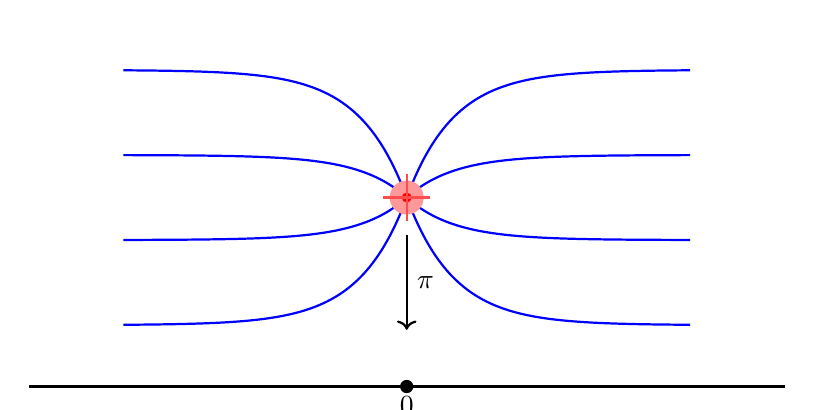
\begin{tikzpicture}[scale=1.2]
				
				% number of sheets
				\def\r{4}
				
				% --- Codomain line ---
				\draw[thick] (-4,-2) -- (4,-2);
%				\node[right] at (4,-2) {$\mathbb{R}$};
				
				% mark origin in base
				\fill (0,-2) circle (2pt);
				\node[below] at (0,-2) {$0$};
				
				% --- Domain sheets ---
				\foreach \k in {1,...,\r} {
					
					\pgfmathsetmacro{\shift}{(\k - (\r+1)/2)}
					
					% right half
					\draw[blue, thick]
					plot[domain=0:3, samples=100]
					(\x, {0.9*\shift*(1 - exp(-2*\x))});
					
					% left half
					\draw[blue, thick]
					plot[domain=0:3, samples=100]
					(-\x, {0.9*\shift*(1 - exp(-2*\x))});
				}
				
				% --- Fuzzy fat branch point ---
				% translucent disk
				\fill[red!40] (0,0) circle (0.18);
				
				% central solid point
				\fill[red] (0,0) circle (1.5pt);
				
				% small radial strokes (multiplicity r)
				\foreach \k in {1,...,\r} {
					\pgfmathsetmacro{\angle}{360/\r * \k}
					\draw[red!70, thick]
					(0,0) -- ({0.25*cos(\angle)}, {0.25*sin(\angle)});
				}
				
				% --- Short projection arrow ---
				\draw[->, thick]
				(0,-0.4) -- (0,-1.4)
				node[midway, right] {$\pi$};
				
			\end{tikzpicture}
		\end{figure}
		Hence, finite locally free is not enough to give us covering maps.
	\end{example}
	The issue is that our definition still allows for branching to happen, whose main cause is typically the existence of nilpotents in the fiber. To remove that, we have to enforce it by hand, fiber-by-fiber.
	\begin{definition}
		A ring homomorphism $\varphi : R\to S$ is \textit{unramified at prime} $\ideal{p} \subseteq S$ if (let $\ideal{q} = \varphi^{-1}\ideal{p}$)
		\begin{enumerate}
			\item {$S$ is a finitely presented $R$-algebra,}
			\item {$\ideal{m}_{\ideal{q}}S_{\ideal{p}}$ is the maximal ideal of $S_{\ideal{p}}$, i.e. $\ideal{m}_{\ideal{q}}S_{\ideal{p}} = \ideal{m}_{\ideal{p}}$,}
			\item {the resulting field extension $\kappa(\ideal{p})/\kappa(\ideal{q})$ is a separable extension.}
		\end{enumerate}
		Otherwise we call it \textit{ramified at $\ideal{p}$}. If it is unramified at each prime, then we just call it \textit{unramified}.
	\end{definition}
	Observe that the map $\varphi $ of Example \ref{E-Finite locally free are NOT local isomorphisms} is ramified at origin (the second condition is not true). So perhaps we should demand that $\varphi : R\to S$ be finite unramified and locally free in order to define local isomorphisms.
	\begin{remark}
		It is to be noted that finite unramified morphisms are still not exactly the notion of local isomorphism that we are looking for. Indeed, $R\to R/I$ for a finitely presented ideal is a finite unramified morphism, but far from what we would consider a local isomorphism (consider $R = k[x,y]$ and $I = (x-y^{2})$) as the corresponding map is just the inclusion of $V(I)$ into $\spec{R}$, not even surjective. 
	\end{remark}
	How can we remove this case? Recall that the quotient $R \to R/I$ is almost never flat and finite locally free maps are flat. This is our cue to define the following.
	\begin{definition}
		A ring homomorphism $\varphi : R\to S$ is said to be \textit{\'etale }if it is unramified and flat.
	\end{definition}
	A closely related notion to \'etale is that of Nisnevich homomorphism.
	\begin{definition}
		A ring homomorphism $R\to S$ is said to be \textit{Nisnevich} if it is \'etale and for each $\ideal{q} \in \spec{R}$, there exists a prime $\ideal{p}$ in the fiber $S\tens_{R} \kappa(\ideal{q})$ in $\spec{S}$ such that the induced map $\kappa(\ideal{q}) \to \kappa(\ideal{p})$ is an isomorphism.
	\end{definition}
	\begin{remark}
		If $R$ and $S$ are noetherian, then since finite locally free and finitely presented flat are equivalent, therefore in such a case an \'etale map is a finite locally free unramified homomorphism.
	\end{remark}
	Let $R$ be a ring and $f\in R$. Observe that $R\to R_f$ is an \'etale map. Moreover, if $R_f,R_g$ covers $R$ (note we can always refine any cover of $R$ to a covering by two basic opens), then the map $R \to R_f\oplus R_g$ is also \'etale. This tells us that \'etale maps in general can act as a generalized notion of local isomorphisms of $R$. Hence, we can define the following.
	\begin{definition}
		An \textit{affine \'etale cover} of $R$ is an $R$-algebra $\varphi  : R\to S$ such that it is \'etale and the map $\spec{S} \to \spec{R}$ is surjective. 
	\end{definition}
	\begin{remark}\label{R-Etale covers are faithfully flat}
		Very importantly, an affine \'etale cover is in particular a faithfully flat morphism (flat and surjective on spec).
	\end{remark}
	Using this we may now define notion of fiber bundles, just akin to how we do it in topology.
	\begin{definition}
		An $k$-algebra homomorphism $\varphi :R\to S$ is said to be an \textit{algebraic fibre bundle with fiber $k$-algebra }$A$ if there exists an affine \'etale cover of $R$, denoted $R\to R^{\prime}$, together with a prescribed isomorphism $ R^{\prime}\tens_{R} S \isom R^{\prime}\tens_{k} A$:
		% https://q.uiver.app/#q=WzAsNixbMSwxLCJSXlxccHJpbWUiXSxbMiwxLCJSIl0sWzIsMCwiUyJdLFsxLDAsIlNeXFxwcmltZSJdLFswLDAsIkEiXSxbMCwxLCJrIl0sWzEsMl0sWzEsMCwiXFx0ZXh0e1xcJ2V0YWxlIGNvdmVyfSJdLFswLDNdLFsyLDNdLFszLDEsIiIsMSx7InN0eWxlIjp7Im5hbWUiOiJjb3JuZXItaW52ZXJzZSJ9fV0sWzUsMF0sWzUsNF0sWzQsM10sWzMsNSwiIiwxLHsic3R5bGUiOnsibmFtZSI6ImNvcm5lci1pbnZlcnNlIn19XV0=
		\[\begin{tikzcd}[cramped]
			A & {S^\prime} & S \\
			k & {R^\prime} & R
			\arrow[from=1-1, to=1-2]
			\arrow["\ulcorner"{anchor=center, pos=0.125, rotate=-90}, draw=none, from=1-2, to=2-1]
			\arrow["\ulcorner"{anchor=center, pos=0.125}, draw=none, from=1-2, to=2-3]
			\arrow[from=1-3, to=1-2]
			\arrow[from=2-1, to=1-1]
			\arrow[from=2-1, to=2-2]
			\arrow[from=2-2, to=1-2]
			\arrow[from=2-3, to=1-3]
			\arrow["{\text{\'etale cover}}", from=2-3, to=2-2]
		\end{tikzcd}.\]
	\end{definition}
	We may define a topology on category of $k$-algebras $\cat{Ring}_{/k}$ as follows.
	\begin{construct}
		For each ring $R \in \cat{Ring}_{/k}$, define $\cat{C}(R) = \{\{\varphi: R\to S\}\;\vert\;\varphi\text{ is an affine \'etale cover}\}$. That is, each element of $\cat{C}(R)$ is a affine \'etale cover of $R$. We claim that $\cat{C}$ is a basis for a Grothendieck topology on $\cat{Ring}_{/k}$. Indeed, this would be immediate from stability of \'etale morphisms under base change and compositions. 
	\end{construct}
	\begin{proposition}
		Unramified and flat morphisms are stable under composition and base change. Hence so is \'etale.
	\end{proposition}
	
	
%	\textbf{TODO : \'Etale coverings, algebraic fiber bundles and triviality of naive covers in Zariski topology.}
	We now want to study \'etale homomorphisms. To this end, the module of K\"ahler differentials is indispensable. 
	\section{K\"ahler differentials}
	How can we differentiate elements of an arbitrary ring just like we do for polynomial rings? Let us try to formulate the process of differentiation of polynomials.
	\begin{remark}
		Let $f$ be a polynomial in one variable over a field $k$. The derivative is defined as the limit $f^{\prime}(y) = \ulim_{x\to y}\frac{f(x)-f(y)}{x-y}$. Observe that the second order Taylor series of $f$ is of the form $f(y) = f(x) + (x-y)f^{\prime}(y) + (x-y)^{2}h(y)$ for some $h$. Hence, consider $f(x)-f(y) \in k[x,y]$. Then the the derivative is given by the class of $f(x)-f(y)$ in $(x-y)/(x-y)^{2}$. We can generalize this to an arbitrary ring $R$ as follows. First observe that $k[x,y] \isom k[x]\tens_{k}k[x]$ under which, $f(x)-f(y)\mapsto f\tens 1 - 1\tens f$ and $x-y \mapsto x\tens 1 - 1\tens x$. Let $I = (x\tens 1- 1\tens x)$ and observe that this is also the kernel of the multipliciation map $k[x]\tens_{k}k[x] \to k[x]$ and note that $f\tens 1 - 1\tens f \in I$. It follows that the derivative is the image of $f\tens 1 - 1\tens f$ in $I/I^{2}$. Moreover, note that $I/I^{2}$ is the $k[x]$-module of all derivatives of each polynomial $f(x)\in  k[x]$.
	\end{remark}
	We can now easily generalize this to arbitrary rings.
	\begin{definition}
		Let $R \to S$ be an $R$-algebra. The module of \textit{K\"ahler differentials} $\Omega_{S/R}$ is the $S$-module $I/I^{2}$ where $I$ is the kernel of the multiplication map $S\tens_{R} S \to S$.
	\end{definition}
	By previous, we can immediately calculate $\Omega_{k[x]/k}$ as a free $k[x]$-module of rank 1, generated by $x\tens 1-1\tens x$.
	\subsection{Universal property}
	There is a universal property satisfied by $\Omega_{S/R}$, which we now discuss. First, revisiting the example of $S=k[x]$, observe that we have a function $d : k[x]\longrightarrow I/I^{2}$ given by $f(x)\mapsto f\tens 1 - 1\tens f$. But this is not a $k$-linear homomorphism, it is a $k$-deriviation.
	\begin{definition}
		Let $R \to S$ be an $R$-algebra and $M$ be an $S$-module. An \textit{$R$-derivation of $S$ valued in $M$} is a function $D : S\to M$ such that $D(s_1 + s_2) = D(s_1) + D(s_2)$, $D(s_1s_2) = s_1D(s_2) + s_2D(s_1)$ and $D(r) = 0$ for all $r\in R$. The collection of all $R$-derivations of $S$ valued in $M$ is denoted by $\Der_{R}(S,M)$. This is an $S$-module.
	\end{definition}
	Observe that for any $R\to S$, the map $d : S \to \Omega_{S/R}$, $s\mapsto s\tens 1 - 1\tens s$ is an $R$-derivation of $S$ valued in $\Omega_{S/R}$. 
	\begin{proposition}
		Let $R\to S$ be an $R$-algebra and $d : S \to \Omega_{S/R}$ be the derivation $s\mapsto 1\tens s - s\tens 1$. For any $S$-module $M$ and any $R$-derivation $D :S\to M$, there exists a unique $S$-linear homomorphism $f : \Omega_{S/R} \to M$ such that the following commutes
		% https://q.uiver.app/#q=WzAsMyxbMCwxLCJTIl0sWzAsMCwiXFxPbWVnYV97Uy9SfSJdLFsxLDAsIk0iXSxbMCwyLCJEIiwyXSxbMCwxLCJkIl0sWzEsMiwiZiIsMCx7InN0eWxlIjp7ImJvZHkiOnsibmFtZSI6ImRhc2hlZCJ9fX1dXQ==
		\[\begin{tikzcd}[cramped]
			{\Omega_{S/R}} & M \\
			S
			\arrow["f", dashed, from=1-1, to=1-2]
			\arrow["d", from=2-1, to=1-1]
			\arrow["D"', from=2-1, to=1-2]
		\end{tikzcd}.\]
	\end{proposition}
	\begin{proof}
		Recall for any $S$-module $M$, we can construct an $S$-algebra $S*M$ which exhibits $M$ as an ideal with $M^{2} = 0$. Indeed, the underlying $S$-module is $S\oplus M$ and the $S$-algebra structure is $(s_1+m_1) \cdot (s_2+m_2) = s_1s_2 + (s_1m_2 + s_2m_1)$. Using this, we first construct the following morphism 
		\begin{align*}
			\varphi_{D} : S\tens_{R} S &\longrightarrow S*M\\
								s_1\tens s_2 &\longmapsto s_1s_2 + s_1Ds_2.
		\end{align*} 
		A simple calculation shows that $\varphi_{D}$ restricted to $I$ maps onto $M$ such that $\varphi_{D}(I^{2}) = 0$. This gives us the homomorphism 
		\begin{align*}
			\varphi_{D} : I/I^{2} = \Omega_{S/R} \longrightarrow M.
		\end{align*}
		We claim that $\varphi_{D}$ works for us. Indeed, $\varphi_{D}\circ d(s) = \varphi_{D} (1\tens s - s\tens 1) = (s+Ds) - (s+0) = Ds$. 
	\end{proof}
	\begin{corollary}
		Let $R\to S$ be an $R$-algebra and $M$ be any $S$-module. Then there is a natural isomorphism of $S$-modules
		\begin{align*}
			\homset{S}{\Omega_{S/R}}{M} \isom \Der_{R}(S,M).
		\end{align*}
		\qed
	\end{corollary}
	\begin{corollary}
		If $R\to S$ is surjective, then $\Omega_{S/R} = 0$.
	\end{corollary}
	\begin{proof}
		Suffices to show that any $R$-derivation $D : S\to M$ is 0. Indeed, as any $s\in S$ is in the image of $R$ and $D(r) = 0$, we are done.
	\end{proof}
	\begin{example}\label{E-Polynomials are smooth}
		Let $S = R[x_1,\dots,x_n]$. Observe that $\Omega_{S/R}$ is generated by $df$ for $f\in S$ polynomials. We claim that $\Omega_{S/R}$ is freely generated by the $n$ elements $dx_i$. Indeed, for any $df \in \Omega_{S/R}$, writing $f = \sum_{I}a_Ix_1^{i_1}\dots x_n^{i_n}$ gives $df = \sum_{I}a_I \sum_{i=1}^{n} g_i(x_1,\dots,\hat{x}_i,\dots,x_n) dx_i$ for some polynomial $g_i$ in $n$ variables. This clearly shows that $dx_i$ generate $\Omega_{S/R}$ and are free generators as well, since $\sum_{i}g_idx_i = 0$ implies $dg = 0$ for some polynomial $g$. It is then immediate that $g = 0$ as each of its partial derivative is. In particular, we have
		\begin{align*}
			\Omega_{S/R} = Sdx_1\oplus \dots \oplus Sdx_n.
		\end{align*}
	\end{example}
	\subsection{Maps and exact sequences of differentials}
	We now wish to study how K\"ahler differentials behave under morphism of rings. In this, there are two cases of morphisms to consider; 
	% https://q.uiver.app/#q=WzAsMyxbMCwwLCJCIl0sWzAsMSwiQSJdLFsxLDAsIkMiXSxbMSwwXSxbMSwyXSxbMCwyXV0=
	\[\begin{tikzcd}[cramped]
		B & C \\
		A
		\arrow[from=1-1, to=1-2]
		\arrow[from=2-1, to=1-1]
		\arrow[from=2-1, to=1-2]
	\end{tikzcd}\]
	one where $B\to C$ is arbitrary and one where it is surjective. Note that in general the diagram 
	% https://q.uiver.app/#q=WzAsNCxbMCwwLCJSIl0sWzAsMSwiUl5cXHByaW1lIl0sWzEsMSwiU15cXHByaW1lIl0sWzEsMCwiUyJdLFszLDJdLFsxLDJdLFswLDFdLFswLDNdXQ==
	\[\begin{tikzcd}
		R & S \\
		{R^\prime} & {S^\prime}
		\arrow[from=1-1, to=1-2]
		\arrow[from=1-1, to=2-1]
		\arrow[from=1-2, to=2-2]
		\arrow[from=2-1, to=2-2]
	\end{tikzcd}\]
	leads to a morphism on differentials over $S\to S^{\prime}$:
	% https://q.uiver.app/#q=WzAsNCxbMCwwLCJTIl0sWzAsMSwiU15cXHByaW1lIl0sWzEsMCwiXFxPbWVnYV97Uy9SfSJdLFsxLDEsIlxcT21lZ2Ffe1NeXFxwcmltZS9SXlxccHJpbWV9Il0sWzAsMl0sWzEsM10sWzAsMV0sWzIsM11d
	\[\begin{tikzcd}[cramped]
		S & {\Omega_{S/R}} \\
		{S^\prime} & {\Omega_{S^\prime/R^\prime}}
		\arrow[from=1-1, to=1-2]
		\arrow[from=1-1, to=2-1]
		\arrow[from=1-2, to=2-2]
		\arrow[from=2-1, to=2-2]
	\end{tikzcd}.\]
	We study this homomorphism of differentials. Observe that if $S\to S^{\prime}$ is surjective, then since any generator of $\Omega_{S^{\prime}/R^{\prime}}$ is $d^{\prime}s^{\prime}$ and $s^{\prime}$ is in image of $S\to S^{\prime}$, the following result follows.
	\begin{lemma}\label{L-Surj implies surj on differentials}
		If $S\to S^{\prime}$ is surjective, then $\Omega_{S/R} \to \Omega_{S^{\prime}/R^{\prime}}$ is surjective. \qed
	\end{lemma}
	The module $\Omega_{S/R}$ acts as the relative cotangent bundle for the homomorphism $R\to S$. With this in mind, we first have the following sequence.
	\begin{lemma}[Relative cotangent sequence]\label{L-Relative cotangent sequence}
		Consider the diagram of $A$-algebras
		% https://q.uiver.app/#q=WzAsMyxbMCwxLCJBIl0sWzEsMCwiQiJdLFsxLDEsIkMiXSxbMCwyXSxbMSwyXSxbMCwxXV0=
		\[\begin{tikzcd}
			& B \\
			A & C
			\arrow[from=1-2, to=2-2]
			\arrow[from=2-1, to=1-2]
			\arrow[from=2-1, to=2-2]
		\end{tikzcd}.\]
		Then we have an exact sequence
		\begin{align*}
			C\tens_{B} \Omega_{B/A} \longrightarrow \Omega_{C/A} \longrightarrow\Omega_{C/B}\longrightarrow0.
		\end{align*}
	\end{lemma}
	\begin{proof}
		Surjectivity follows from Lemma \ref{L-Surj implies surj on differentials}. The map $C\tens_{B} \Omega_{B/A} \to \Omega_{C/A}$ is given by $c\tens d_{B/A}b \mapsto cd_{C/A}b$. As the map $\Omega_{C/A} \to \Omega_{C/B}$ is given by $d_{C/A}c \mapsto d_{C/B}c$, therefore the whole composite is given by $c\tens db \mapsto cd_{C/B}(b) = 0$. On the other hand, if $\alpha = \sum_{i}c_i d_{C/A}c_i^{\prime} \in \Omega_{C/A}$ maps to $0$ in $\Omega_{C/B}$, then $\sum_{i}c_i d_{C/B}c_i^{\prime} = 0$, i.e. each $c_i^{\prime}$ is in the image of $B$ in $C$. Completing the proof.
	\end{proof}
	\begin{lemma}[Relative conormal sequence]
		Consider the diagram of $R$-algebras
	% https://q.uiver.app/#q=WzAsMyxbMCwxLCJSIl0sWzEsMCwiUyJdLFsxLDEsIlNeXFxwcmltZSJdLFsxLDIsIiIsMCx7InN0eWxlIjp7ImhlYWQiOnsibmFtZSI6ImVwaSJ9fX1dLFswLDFdLFswLDJdXQ==
	\[\begin{tikzcd}
		& S \\
		R & {S^\prime}
		\arrow[two heads, from=1-2, to=2-2]
		\arrow[from=2-1, to=1-2]
		\arrow[from=2-1, to=2-2]
	\end{tikzcd}\]
	where $S\to S^{\prime}$ is surjective with $I = \Ker{S\to S^{\prime}}$. Then we have an exact sequence
	% https://q.uiver.app/#q=WzAsNCxbMiwwLCJcXE9tZWdhX3tTXlxccHJpbWUvUn0iXSxbMSwwLCJTXlxccHJpbWVcXHRlbnNfU1xcT21lZ2Ffe1MvUn0iXSxbMywwLCIwIl0sWzAsMCwiSS9JXjIiXSxbMSwwXSxbMCwyXSxbMywxXV0=
	\[\begin{tikzcd}
		{I/I^2} & {S^\prime\tens_S\Omega_{S/R}} & {\Omega_{S^\prime/R}} & 0
		\arrow[from=1-1, to=1-2]
		\arrow[from=1-2, to=1-3]
		\arrow[from=1-3, to=1-4]
	\end{tikzcd}\]
	where the map $I/I^2 \to S^{\prime}\tens_{S} \Omega_{S/R}$ is induced by $s\mapsto 1\tens ds$ for $s\in I$. We call $I/I^{2}$ the conormal module.
	\end{lemma}
	\begin{proof}
		Surjection is clear by $\Omega_{S^{\prime}/S} = 0$ (Lemma \ref{L-Surj implies surj on differentials}) and Lemma \ref{L-Relative cotangent sequence}. Exactness at the middle is simple. 
	\end{proof}
	\subsection{Separability}
	Recall that a polynomial $f$ in one variable over a field $k$ is separable if and only if it is coprime to its derivative; $\gen{f,f^{\prime}} = 1$. As we have seen, $\Omega_{S/R}$ can be seen as the module of all derivatives of functions in the $R$-algebra $S$. Further recall that a $k$-algebra $A$ is said to be \textit{finite separable} if it is a finite product of finite separable field extensions $K_i/k$, $A = \prod_{i}K_i$. We now see that $\Omega_{K/k}$ detects separability.
	\begin{theorem}\label{T-Differentials vanish for separable extensions}
		Let $K/k$ be a finite extension. Then the following are equivalent:
		\begin{enumerate}
			\item {$K/k$ is a separable extension.}
			\item {$\Omega_{K/k} = 0$.}
		\end{enumerate}
	\end{theorem}
	\subsection{Finite presentation}
	\begin{proposition}\label{P-FP descends to Differentials}
		If $R\to S$ is a finitely presented morphism, then $\Omega_{S/R}$ is a finitely presented $S$-module.
	\end{proposition}
	
	\subsection{Localization}
	An important observation about differentials is that it is very well-behaved with respect to localizations.
	\begin{proposition}\label{P-Differential localization}
		Let $\varphi : A\to B$ be a ring homomorphism.
		\begin{enumerate}
			\item {If $S\subseteq A$ is a multiplicative set such that $\varphi(S) \subset B^{\times}$, then 
			\begin{align*}
				\Omega_{B/A} \isom \Omega_{B/A[S^{-1}]}.
			\end{align*}
			}
			\item {If $S\subseteq B$ is a multiplicative set, then 
			\begin{align*}
				B[S^{-1}] \tens_{B} \Omega_{B/A} \isom \Omega_{B[S^{-1}]/A}
			\end{align*}
			}
		\end{enumerate}
	\end{proposition}
	
	
	\subsection{Base change}
	Similarly, it is well-behaved with respect to base change as well.
	\begin{proposition}\label{P-Differential Base Change}
		Consider the following pushout square for rings
		% https://q.uiver.app/#q=WzAsNCxbMSwxLCJSIl0sWzAsMSwiUl5cXHByaW1lIl0sWzEsMCwiUyJdLFswLDAsIlNeXFxwcmltZSJdLFsxLDNdLFswLDJdLFswLDFdLFsyLDNdLFszLDAsIiIsMSx7InN0eWxlIjp7Im5hbWUiOiJjb3JuZXItaW52ZXJzZSJ9fV1d
		\[\begin{tikzcd}[cramped]
			{S^\prime} & S \\
			{R^\prime} & R
			\arrow["\ulcorner"{anchor=center, pos=0.125}, draw=none, from=1-1, to=2-2]
			\arrow[from=1-2, to=1-1]
			\arrow[from=2-1, to=1-1]
			\arrow[from=2-2, to=1-2]
			\arrow[from=2-2, to=2-1]
		\end{tikzcd},\]
		i.e. $S^{\prime} = S\tens_{R} R^{\prime}$. Then there is a canonical isomorphism 
		\begin{align*}
			S^{\prime}\tens_{S} \Omega_{S/R} \isom \Omega_{S^{\prime}/R^{\prime}}.
		\end{align*}
	\end{proposition}

	\section{Smooth homomorphisms}
	As we use K\"ahler differentials for studying smoothnes of ring maps, we should perhaps begin our discussion for differentials on unramified map. 
	\subsection{Differentials and ramification}
	\begin{proposition}\label{P-Unramified implies no differentials}
		If $\varphi : R\to S$ is an unramified homomorphism, then $\Omega_{S/R} = 0$.
	\end{proposition}
	\begin{proof}
		Note it suffices to show that $\Omega_{S/R,\ideal{p}} = 0$ for each prime $\ideal{p}$ of $S$. Let $\ideal{p}\in \spec{S}$ and $\ideal{q} = \varphi^{-1}(\ideal{p}) \in \spec{R}$. We get a local homomorphism $\varphi_{\ideal{p}} : R_\ideal{q} \to S_{\ideal{p}}$. By Proposition \ref{P-Differential localization} $ \Omega_{S/R,\ideal{p}} = \Omega_{S_{\ideal{p}}/R} \isom \Omega_{S_{\ideal{p}}/ R_\ideal{q}}$. Thus, we reduce to assuming $\varphi :R\to S$ is a local unramified homomorphism of local rings. Thus, $\ideal{m}_{R}S = \ideal{m}_{S}$, in particular.\\\indent
		By Nakayama lemma, it suffices to show that $\Omega_{S/R}/\ideal{m}_{S}\Omega_{S/R} = 0$. Indeed, we may write this as
		\begin{align*}
			\Omega_{S/R}/\ideal{m}_{S}\Omega_{S/R} = S/\ideal{m}_{R}S \tens_{S} \Omega_{S/R} = K\tens_{S}\Omega_{S/R} 
		\end{align*}
		where $K$ is the residue field of $S$ and let $k$ the resiude field of $R$. Note we have a pushout square 
		% https://q.uiver.app/#q=WzAsNCxbMCwxLCJrIl0sWzEsMSwiUiJdLFsxLDAsIlMiXSxbMCwwLCJLIl0sWzEsMiwiXFx2YXJwaGkiLDJdLFsxLDBdLFsyLDNdLFswLDNdLFszLDEsIiIsMSx7InN0eWxlIjp7Im5hbWUiOiJjb3JuZXItaW52ZXJzZSJ9fV1d
		\[\begin{tikzcd}[cramped]
			K & S \\
			k & R
			\arrow["\ulcorner"{anchor=center, pos=0.125}, draw=none, from=1-1, to=2-2]
			\arrow[from=1-2, to=1-1]
			\arrow[from=2-1, to=1-1]
			\arrow["\varphi"', from=2-2, to=1-2]
			\arrow[from=2-2, to=2-1]
		\end{tikzcd},\]
		indeed, $k \tens_{R} S = R/\ideal{m}_{R}\tens_{R} S = S/\ideal{m}_{R}S = S/\ideal{m}_{S} = K$. Thus, by Proposition \ref{P-Differential Base Change}, 
		\begin{align*}
			K\tens_{S}\Omega_{S/R} = \Omega_{K/k}.
		\end{align*} 
		By Theorem \ref{T-Differentials vanish for separable extensions}, we have $\Omega_{K/k} = 0$. This completes the proof.
	\end{proof}
	\subsection{Smoothness}
	Recall that for a smooth manifold, tangent spaces at each point arranges itself into a vector bundle. This is essentially because of the fact that locally a smooth manifold is diffeomorphic to a connected domain in an Euclidean space. Thus one way of pinning smoothnes down is via the demand that (co)tangent spaces must have same rank locally, i.e. locally we must always have $n$-sections of the family of (co)tangent spaces. Using this, it is now a simple job to define smooth homomorphisms. For posterity, recall the following conclusion of Zariski descent.
	\begin{theorem}
		Let $R$ be a noetherian ring and $P$ be a finitely presented $R$-module. Then the following are equivalent:
		\begin{enumerate}
			\item {$P$ is a projective $R$-module.}
			\item {$P$ is a locally free $R$-module.}
			\item {$P$ is a flat $R$-module.}
		\end{enumerate}
	\end{theorem}
	\begin{definition}
		A homomorphism $\varphi: R\to S$ is \textit{smooth} if $\varphi$ is finitely presented $R$-algebra morphism, flat and $\Omega_{S/R}$ is a projective $S$-module. 
	\end{definition}
	Recall from Proposition \ref{P-FP descends to Differentials} that for a smooth homomorphism, $\Omega_{S/R}$ is also finitely presented. We first immediately see the following
	\begin{lemma}
		If $R\to S$ is \'etale, then it is smooth. 
	\end{lemma}
	\begin{proof}
		An \'etale map is flat and unramified, so finitely presented and flat. Further by Proposition \ref{P-Unramified implies no differentials}, it follows that $\Omega_{S/R} = 0$, i.e. it is projective.
	\end{proof}
	\begin{example}
		The map $R\to  S= R[x_1,\dots,x_n]$ is smooth. Indeed, $S$ is finitely presented as an $R$-algebra and $\Omega_{S/R} = Sdx_1\oplus \dots \oplus Sdx_n$, making it free thus projective $S$-module.
	\end{example}
	While this definition of smoothness is geometrically clear, it is usually very difficult to work with. To that end, we can equivalently characterize smooth morphisms via following criterion.
	\subsection{Formal smoothness}
	\begin{definition}
		A ring homomorphism $R\to S$ is said to be \textit{formally smooth} if given any $R$-algebra $A$ and a square-zero ideal $I \subset A$, any homomorphism $S\to A/I$ extends to a homomorphism $S\to A$:
		% https://q.uiver.app/#q=WzAsNCxbMSwxLCJBIl0sWzAsMSwiUiJdLFswLDAsIlMiXSxbMSwwLCJBL0kiXSxbMCwzXSxbMSwyXSxbMSwwXSxbMiwzXSxbMiwwLCIiLDEseyJzdHlsZSI6eyJib2R5Ijp7Im5hbWUiOiJkYXNoZWQifX19XV0=
		\[\begin{tikzcd}[cramped]
			S & {A/I} \\
			R & A
			\arrow[from=1-1, to=1-2]
			\arrow[dashed, from=1-1, to=2-2]
			\arrow[from=2-1, to=1-1]
			\arrow[from=2-1, to=2-2]
			\arrow[from=2-2, to=1-2]
		\end{tikzcd}.\]
	\end{definition}
	We have the following criterion for smoothness.
	\begin{theorem}[Formal criterion for smoothness]
		Let $R\to S$ be an $R$-algebra. Then the following are equivalent:
		\begin{enumerate}
			\item {$R\to S$ is smooth.}
			\item {$R\to S$ is a finitely presented, formally smooth $R$-algebra.}
		\end{enumerate}
	\end{theorem}
%	\begin{proof}
%		(1. $\Rightarrow$ 2.) It suffices to show formal smoothness of $R\to S$. 
%	\end{proof}
	
	
	\begin{lemma}[Composite]\label{L-Smooth stable under composites}
		If $R\to S$ and $S\to T$ are smooth, then the composite $R\to T$ is smooth.
	\end{lemma}
	\begin{proof}
		Immediate from formal smoothness.
	\end{proof} 
	\begin{lemma}[Base change]\label{L-Base change for smooth}
		Consider the pushout 
		% https://q.uiver.app/#q=WzAsNCxbMCwxLCJSXlxccHJpbWUiXSxbMSwxLCJSIl0sWzEsMCwiUyJdLFswLDAsIlNeXFxwcmltZSJdLFsxLDJdLFsxLDBdLFswLDNdLFsyLDNdLFszLDEsIiIsMSx7InN0eWxlIjp7Im5hbWUiOiJjb3JuZXItaW52ZXJzZSJ9fV1d
		\[\begin{tikzcd}[cramped]
			{S^\prime} & S \\
			{R^\prime} & R
			\arrow["\ulcorner"{anchor=center, pos=0.125}, draw=none, from=1-1, to=2-2]
			\arrow[from=1-2, to=1-1]
			\arrow[from=2-1, to=1-1]
			\arrow[from=2-2, to=1-2]
			\arrow[from=2-2, to=2-1]
		\end{tikzcd}.\]
		If $R\to S$ is smooth, then $R^{\prime}\to S^{\prime}$ is smooth.
	\end{lemma}
	\begin{proof}
		Finite presentation is immediate. Formal smoothness follows from universal property of pushouts.
	\end{proof}
	\begin{lemma}[\'Etale locality of smoothness]
		Let $\varphi : R\to S$ be an $R$-algebra. Then the following are equivalent:
		\begin{enumerate}
			\item {For any affine \'etale cover $R\to R^{\prime}$ of $R$, the map $R^{\prime} \to S^{\prime} = S\tens_{R}R^{\prime}$ is smooth:
			% https://q.uiver.app/#q=WzAsNCxbMSwxLCJSIl0sWzEsMCwiUyJdLFswLDEsIlJeXFxwcmltZSJdLFswLDAsIlNeXFxwcmltZSJdLFswLDIsIlxcdGV4dHtcXGZvb3Rub3Rlc2l6ZSBcXCdldGFsZSBjb3Zlcn0iXSxbMCwxXSxbMiwzXSxbMSwzXSxbMywwLCIiLDEseyJzdHlsZSI6eyJuYW1lIjoiY29ybmVyLWludmVyc2UifX1dXQ==
			\[\begin{tikzcd}[cramped]
				{S^\prime} & S \\
				{R^\prime} & R
				\arrow["\ulcorner"{anchor=center, pos=0.125}, draw=none, from=1-1, to=2-2]
				\arrow[from=1-2, to=1-1]
				\arrow[from=2-1, to=1-1]
				\arrow[from=2-2, to=1-2]
				\arrow["{\text{\footnotesize \'etale cover}}", from=2-2, to=2-1]
			\end{tikzcd}.\]
			}
			\item {$R\to S$ is smooth.}
		\end{enumerate}
	\end{lemma}
	\begin{proof}
		The (1. $\Rightarrow$ 2.) is faithfully flat (Remark \ref{R-Etale covers are faithfully flat}) descent for formally smooth homomorphisms. The converse is base change (Lemma \ref{L-Base change for smooth}).
	\end{proof}
	\begin{remark}[Formally unramified and \'etale]\label{R-Formally unramified and etale}
		While not discussed here, one can similarly give the following two definitions; a map $R\to S$ is said to be formally unramified(\'etale) if for all $R\to A$ and a square-zero ideal $I \subseteq A$, there exists atmost one (unique) extension $S\to A$ as in the diagram
		\[\begin{tikzcd}[cramped]
			S & {A/I} \\
			R & A
			\arrow[from=1-1, to=1-2]
			\arrow[dashed, from=1-1, to=2-2]
			\arrow[from=2-1, to=1-1]
			\arrow[from=2-1, to=2-2]
			\arrow[from=2-2, to=1-2]
		\end{tikzcd}.\]
		In-fact, we then have the following results.
 	\end{remark}
	\begin{theorem}
		Let $R\to S$ be a $R$-algebra. Then the following are equivalent:
		\begin{enumerate}
			\item {$R\to S$ is  formally unramified (\'etale) finitely presented $R$-algebra.}
			\item {$R\to S$ is unramified (\'etale).}
		\end{enumerate}
	\end{theorem}
%	\subsection{Regularity and smoothness}
	
	\section{Local structure of smooth morphisms}
	Let us document some results which showcases that smooth maps \'etale locally really does behave like smooth maps between manifolds. First, recall that a smooth map of manifolds is a local isomorphism (\'etale) exactly when the map induces an isomorphism on each tangent space (or equivalently on cotangent spaces). We have exactly similar result for rings, \'etale locally.
	\begin{proposition}\label{P-Etale maps induce isomorphisms on cotangent spaces}
		Let $\varphi : (S,\ideal{m}) \to (T,\ideal{n})$ be essentially of finite presentation, local homomorphisms of local $R$-algebras. Further suppose $\varphi$ is formally smooth. Then the following are equivalent:
		\begin{enumerate}
			\item {$\varphi$ is formally \'etale.}
			\item {The map $T\tens_{S}\Omega_{S/R} \to \Omega_{T/R}$ is an isomorphism.}
		\end{enumerate}
	\end{proposition}
	\begin{theorem}
		Let $\varphi : (R,\ideal{m}) \to (T,\ideal{n})$ be essentially of finite presentation, local homomorphisms of local rings. Then the following are equivalent:
		\begin{enumerate}
			\item {$\varphi$ is a formally smooth.}
			\item {There exists a factorization 
			\begin{align*}
				R\to S\to T
				\end{align*}
			where $(S,\ideal{q})$ is the local ring obtained by localization of $R[x_1,\dots,x_n]$ at a prime, $R\to S$ the canonical inclusion and $S\to T$ is a formally \'etale homomorphism.
			}
		\end{enumerate} 
	\end{theorem}
	\begin{proof}
		(1. $\Rightarrow$ 2.) As $\Omega_{T/R}$ is a finitely generated projective $T$-module and $T$ is a local ring, therefore $\Omega_{T/R}$ is finite free, say of rank $n$. Thus $\Omega_{T/R} = Tdt_1\oplus \dots \oplus Tdt_n$ for $t_i \in T$. This gives us a homomorphism $R[x_1,\dots,x_n] \longrightarrow T$, mapping $x_i \mapsto t_i$. Let $\ideal{p}$ be the contraction of $\ideal{n}$, so that localizing the morphism at $\ideal{p}$ gives
		\begin{align*}
			S:= R[x_1,\dots,x_n]_{\ideal{p}} \longrightarrow T_{\ideal{n}} = T.
		\end{align*}
		We claim that this morphism works for the problem. To this end, we need only show that the morphism $S\to T$ is formally \'etale. By Proposition \ref{P-Etale maps induce isomorphisms on cotangent spaces}, it suffices to show that 
		\begin{align*}
			T\tens_{S} \Omega_{S/R} &\longrightarrow \Omega_{T/R}\\
					t\tens ds &\longmapsto tds
		\end{align*}
		is an isomorphism of $T$-modules. Indeed, we have that $1\tens dx_i$ maps to the free generators $dt_i$ of $\Omega_{T/R}$ thus it is surjective and it is injective as it is a surjection onto a finite free module over a local ring (Nakayama lemma). \\\\
		(2. $\Rightarrow$ 1.) Suffices to show that $R\to S$ and $S\to T$ is formally smooth (Lemma \ref{L-Smooth stable under composites}). As $S\to T$ is formally \'etale, so formally smooth (Remark \ref{R-Formally unramified and etale}) and $R\to S$ is an inclusion to a localization of a polynomial algebra (Proposition \ref{P-Differential localization}), so again formally smooth. This completes the proof.
	\end{proof}
	
\end{document}